\section{Reporting errors}
Should anomalies or errors encountered during the execution of the plug-in or the training tool, it is possible to report them ad the following mail address: \href{mailto:gruppoafk15@gmail.com}{gruppoafk15@gmail.com}.

\subsection{Reporting Training tool errors}
In the object field the type of error must be stated in the following way:\\ \centerline{\textbf{[Error][Training tool]}} \\
The body of the mail must contain the  following statements:

\begin{itemize}
	\item operating system version;
	\item training tool version;
	\item detailed explanation of the encountered error.
\end{itemize}

\begin{figure}[H]
\centering
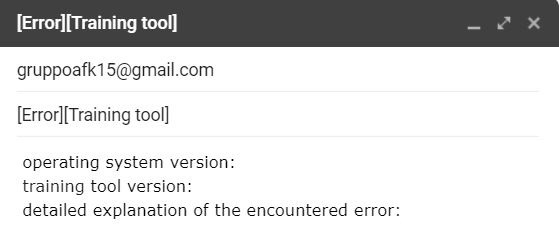
\includegraphics[scale=0.85]{img/mail/tool_mail.png}
\caption{Training tool error mail template}
\end{figure}

\subsection{Reporting Plug-in errors}
To report Plug-in errors instead: the object field has to be compiled as such:\\ \centerline{\textbf{[Error][Plug-in]}} \\
and the body must contain the following statements:
\begin{itemize}
\item Grafana version;
\item plug-in version;
\item browser version;
\item operating system version;
\item  detailed explanation of the encountered.
\end{itemize}

\begin{figure}[H]
\centering
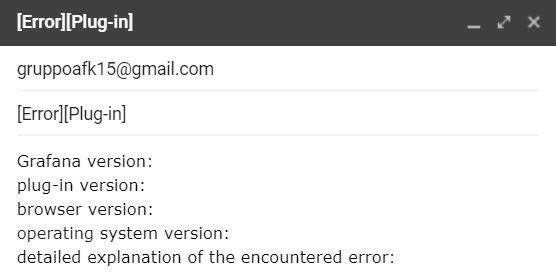
\includegraphics[scale=0.85]{img/mail/plug-in_mail.png}
\caption{Plug-in error mail template}
\end{figure}